% arara: xelatex: { shell : yes }

% kompilace xelatex prezentace.tex
% dokumentace k beameru: http://ftp.cvut.cz/tex-archive/macros/latex/contrib/beamer/doc/beameruserguide.pdf

\RequirePackage[hyphens]{url}

% nastavení formátu prezentace 16:9 
\documentclass[czech,aspectratio=169]{beamer}

\usepackage{polyglossia}
\setmainlanguage{czech}

% nastavení vzhledu 
% další možnosti vzhledu viz https://hartwork.org/beamer-theme-matrix/
\usetheme{Madrid}
\usecolortheme{whale}

% vzhled slajdů vnitřní téma (např. vzhled odrážek)
\useinnertheme{rectangles} %možnosti: default circles rectangles rounded inmargin
% vzhled slajdů vnější téma
\useoutertheme{default} %možnosti: default, miniframes, smoothbars, sidebar, split, shadow, tree, smoothtree, infolines

% zavedeme čvutí modou barvu
\definecolor{CVUT}{HTML}{0065BD}
% čvutí modou použijeme jako hlavní barvu prezentace
\setbeamercolor{structure}{bg=white,fg=CVUT}

% jako font prezentace nadefinujeme oficiální ČVUT písmo Technika -- pokud chcete použít, musíte si font nainstalovat nebo jej nahrát na Overleaf
% https://www.cvut.cz/logo-a-graficky-manual  -- inforek, přihlášení přes celoškolské heslo
%\usepackage{fontspec}
%\setsansfont{Technika-Kniha}

% vypneme navigační panel beamer (pro zapnutí zakomentujeme)
\beamertemplatenavigationsymbolsempty

% vygenerujeme slajdy s poznámkami -- ty si můžete vytisknout a mít je na obhajobu s sebou (pokud zapomenete slova, nebo kdyby nefungovalo promítání z nějakého důvodu)
%\setbeameroption{show notes}

% další balíčky
\usepackage{graphicx}
\usepackage{minted}
\usepackage{csquotes}
\usepackage{multimedia}
\usepackage{hyperref}
\usepackage{tikz}
\usetikzlibrary{chains,fit,shapes}

% Údaje o prezentaci
\title[King Karel -- Logická hra na výuku programování]{King Karel -- Logická hra na výuku programování}
\subtitle{Diplomová práce}
\institute[FIT ČVUT v~Praze]{Fakulta informačních technologií \\ České vysoké učení technické v~Praze}
\author[J. Bittner]{Bc. Jan Bittner \\ Vedoucí práce: Ing. Jan Matoušek}
\date{7. 6. 2022}
\titlegraphic{
\includegraphics[width=.1\textwidth]{assets/slides/logo-cvut}}

\begin{document}
  \begin{frame}
    \titlepage 
    \note{Nezapomenout pozdravit} %tohle je poznámka, ta na slajdu nebude, ale vygeneruje se vedle něj, pokud odkomentujete příkaz výše -- \setbeameroption{show notes} 
  \end{frame}
  
  %\begin{frame}
  %  \tableofcontents %generuje se automaticky z section, subsection, subsubsection
  %\end{frame}

  \begin{frame}{Motivace}
    \begin{center}
      \begin{itemize}
        \item vzdělávání
        \item děti a mladiství
        \item gamifikace
        \item osobní zkušenosti
      \end{itemize}
    \end{center}
  \end{frame}

  \begin{frame}{Cíle práce}
    \begin{itemize}
      \item analýza podobných her na výuku programování
      \item analýza technologií
      \item návrh architektury, hry a~herní logiky
      \item implementace herního prototypu
      \item uživatelské testování
    \end{itemize}
  \end{frame}

  \begin{frame}{Technologie}
    \begin{itemize}
      \item \textbf{Dart, Flutter} -- klientská aplikace
      \item \textbf{C\#, ASP.NET Web API} -- serverová aplikace
      \item \textbf{Clean Architecture} -- architektura
      \item \textbf{PostgreSQL} -- databáze
    \end{itemize}
  \end{frame}

  \begin{frame}{Ukázka hry}
    \begin{center}
      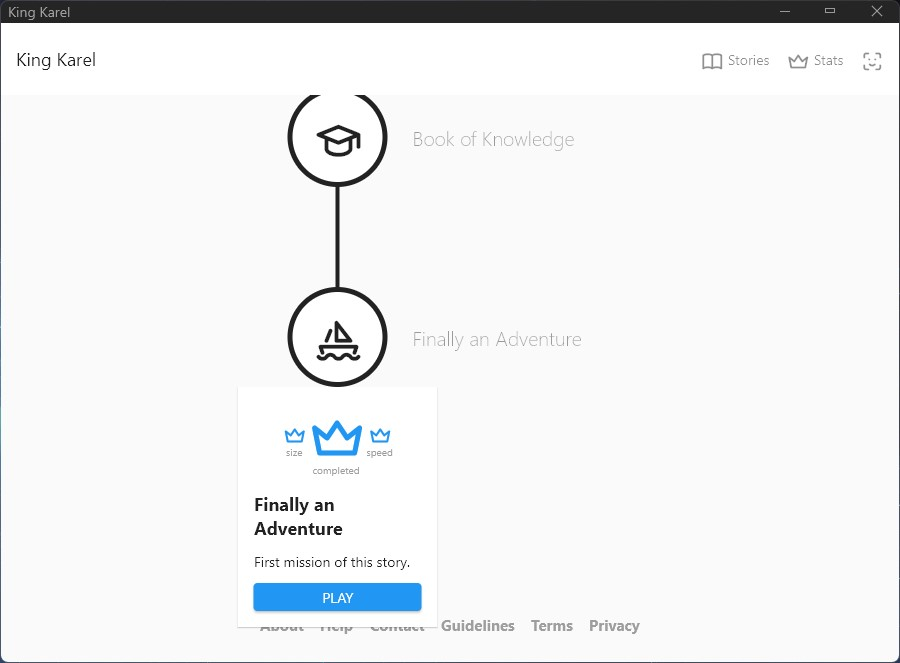
\includegraphics[width=.6\textwidth]{assets/slides/kingkarel_story}
    \end{center}
  \end{frame}

  \begin{frame}{Ukázka hry}
    \begin{center}
      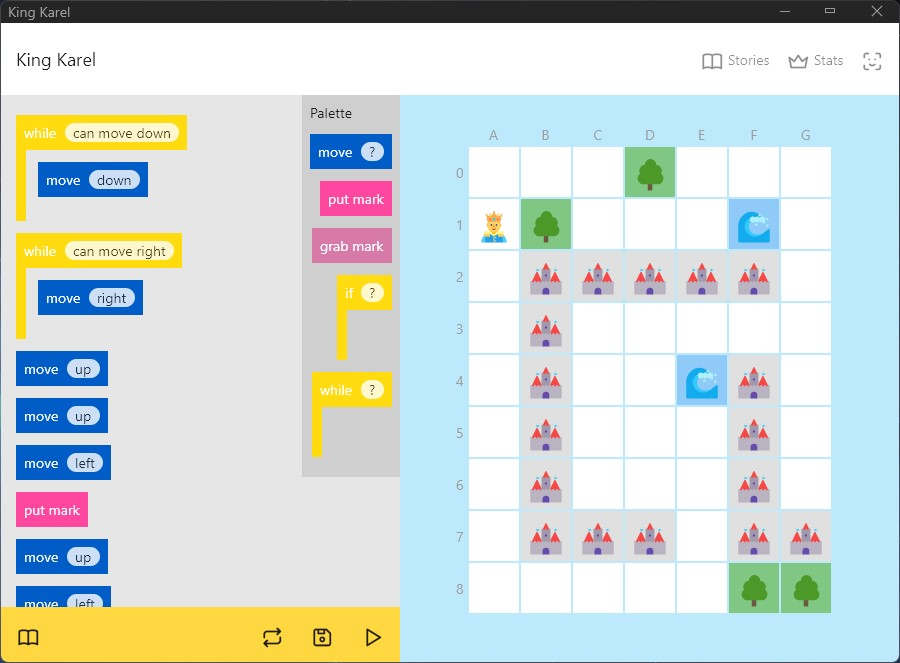
\includegraphics[width=.6\textwidth]{assets/slides/kingkarel_game}
    \end{center}
  \end{frame}

  \begin{frame}{Ukázka hry}
    \begin{center}
      ... video
    \end{center}
  \end{frame}

  \begin{frame}{Clean Architecture}
    \begin{center}
      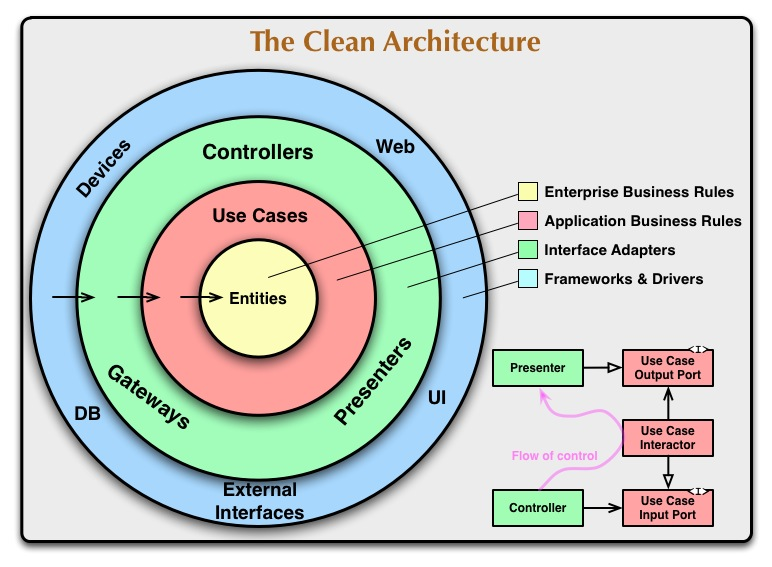
\includegraphics[width=.4\textwidth]{assets/slides/logo-clean-architecture}
    \end{center}
      \begin{center}
        {\large ``The way you keep software soft is
      to leave as many options open as possible,
      for as long as possible.
      What are the options that we need to leave open?\\
      They are the details
      that don’t matter.''}
      \vskip5mm
      --- Robert C. Martin, Clean Architecture
      \end{center}
  \end{frame}

  \begin{frame}{Client}
    \begin{center}
      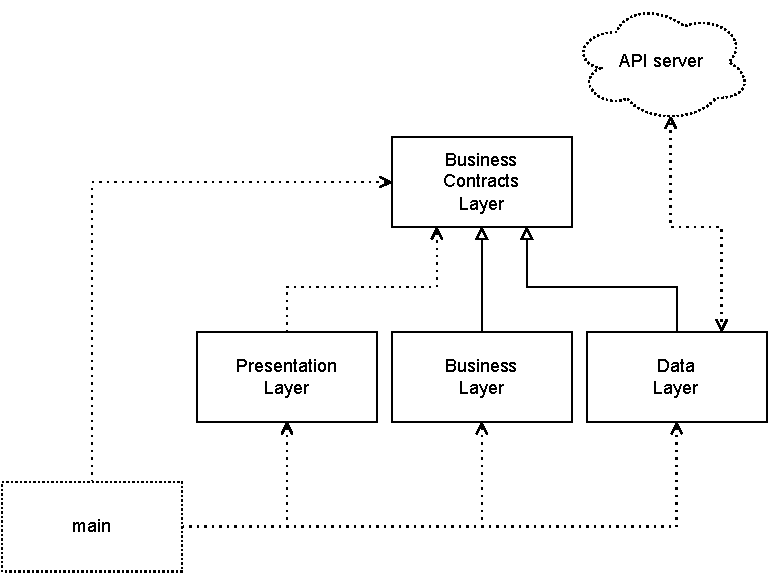
\includegraphics[width=.57\textwidth]{assets/slides/clientarchitecture}
    \end{center}
  \end{frame}

  \begin{frame}{Server}
    \begin{center}
      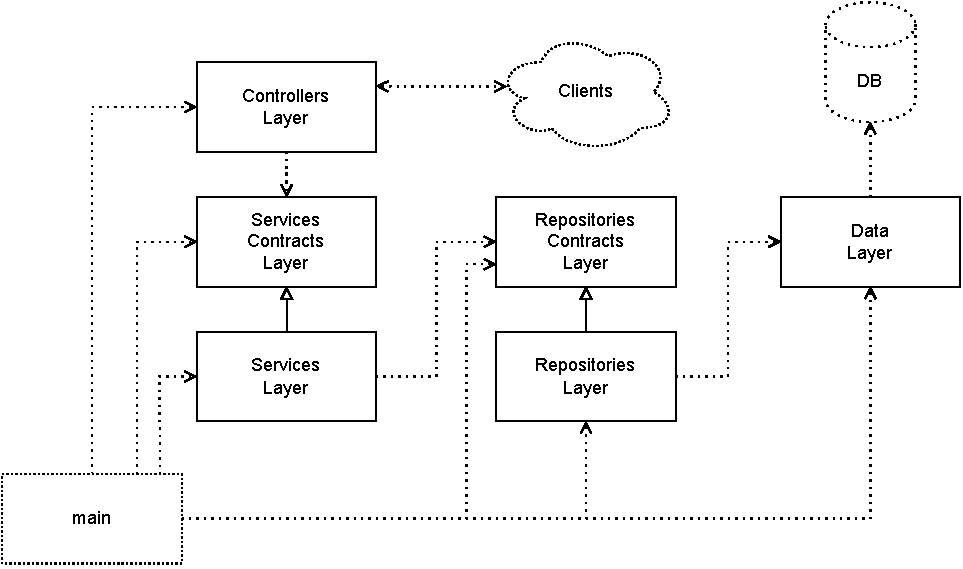
\includegraphics[width=.7\textwidth]{assets/slides/serverarchitecture}
    \end{center}
  \end{frame}

  \begin{frame}{Shrnutí}
    \begin{itemize}
      \item Všechny cíle splněny.
      \item Návrh a~vytvoření funčního prototypu.
      \item Spokojenost uživatelů při testování.
      \item Mnoho možností rozšíření a~adaptace.
    \end{itemize}
  \end{frame}

  \begin{frame}{Zdroje}
    \begin{itemize}
      \item MARTIN, Robert C. \emph{The Clean Architecture} [online]. 2012 [cit. 2022-06-01]. Dostupné z: \url{https://blog.cleancoder.com/uncle-bob/2012/08/13/the-clean-architecture.html}.
      \item MARTIN, Robert C. \emph{Clean Architecture: A~Craftsman’s Guide to Soft-ware Structure and Design}. Prentice Hall, 2018, s. 140. ISBN 0134494164. Dostupné z: \url{https://www.amazon.com/Clean-Architecture-Craftsmans-Software-Structure-ebook/dp/B075LRM681}. 
    \end{itemize}
  \end{frame}

  \begin{frame}{Děkuji za pozornost}
    \begin{center}
      Prostor pro dotazy.
    \end{center}
  \end{frame}

  \begin{frame}[noframenumbering]{Otázky oponenta}
    Otázka první:
    Existuje nějaký časový rámec, kdy by měla být hra King Karel dostupná pro~veřejnost?

    \vfill

    Přesný časový rámec zatím není znám.
    Prototyp však prokázal, že projekt má smysl a proto bude jeho vývoj pokračovat.
    K plnému vydání hry bude potřeba zejména vylepšit uživatelské rozhraní a přidat další zajímavé prvky.
    Jelikož bude projekt vyvíjen ve volném čase, očekávám první veřejnou verzi do konce roku 2023.
  \end{frame}

  \begin{frame}[noframenumbering]{Otázky oponenta}
    Otázka druhá:
    Existuje editor levelů a bude případně dostupný i pro uživatele?

    \vfill

    Odpověď:
    Ne všechny funkcionality jsou v prototypu implementovány, ale přesto je jich řada navíc popsána v kapitole 2.1.7 Future Features.
    Kapitola 2.1.7.4 Creator Screen přímo zmiňuje funkcionalitu totožnou s \enquote{editorem levelů}.
    Zda bude tento editor, respektive vytváření obsahu obecně, dostupný všem koncovým uživatelům, zatím není jisté.
  \end{frame}
\end{document}
